\clearpage

\paragraph{Soggetto 1}~

\vspace{1cm}

\noindent Per verificare le prestazioni e il funzionamento dei moduli progettati, sono state effettuate alcune misure su un soggetto maschio, di 55 anni con carnagione chiara. Il soggetto si trovava in condizioni di riposo.

\vspace{0.5cm}

\noindent Di seguito sono riportati i risultati ottenuti utilizzando il sensore \textbf{MAX86916}, su una finestra temporale di 10 secondi, in vari siti di misura.

\subparagraph{Polpastrello indice sinistro}

Il polpastrello rappresenta il sito di misura più utilizzato poiché permette di ottenere ottimi segnali PPG ed è facilmente indossabile. Come si può notare in figura \ref{fig:soggetto1_MAX86916_polpastrello}, tutte le misure presentano una buona e distinguibile componente AC. Infatti, è possibile osservare sia il picco sistolico sia il picco diastolico anche con la luce verde e blu. Le acquisizioni con la luce verde e blu presentano un andamento più \textit{smooth}. Questa caratteristica è determinata dalla minore penetrazione della luce verde-blu, che rende le misure meno soggette ad interferenze dovute a movimenti, anche minimi, del soggetto. Il segnale con un'ampiezza maggiore è risultato essere quello del LED verde. Contando i picchi presenti, e moltiplicandoli per un fattore 6, è possibile effettuare una stima della frequenza cardiaca del soggetto. In questa misura, si possono individuare 12 picchi, stimando una frequenza cardiaca di 72 battiti al minuto.

\begin{figure}[h]
	\centering
	\includegraphics[width=1\linewidth]{ImageFiles/Misure Preliminari/Soggetto 1/MAX86916/polpastrello_ired}
	\includegraphics[width=1\linewidth]{ImageFiles/Misure Preliminari/Soggetto 1/MAX86916/polpastrello_red}
	\includegraphics[width=1\linewidth]{ImageFiles/Misure Preliminari/Soggetto 1/MAX86916/polpastrello_green}
	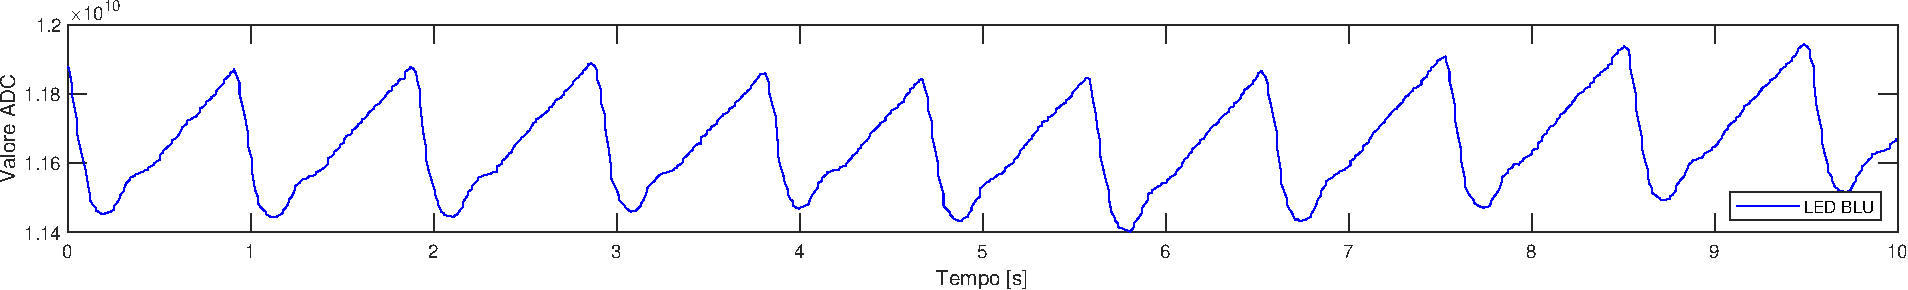
\includegraphics[width=1\linewidth]{ImageFiles/Misure Preliminari/Soggetto 1/MAX86916/polpastrello_blu}
	\caption{Soggetto 1 - Segnali PPG acquisiti sul polpastrello del dito indice sinistro con il sensore MAX86916.}
	\label{fig:soggetto1_MAX86916_polpastrello}
\end{figure}

\clearpage

\subparagraph{Lobo orecchio destro}

In figura \ref{fig:soggetto1_MAX86916_lobo} sono riportate le misure effettuate sul lobo dell'orecchio destro. I segnali risultano buoni anche in questo sito di misura con tutti e quattro i LED. Utilizzando il prototipo realizzato, il sito non è risultato comodo per effettuare le misure. Tuttavia, come già analizzato nel capitolo \ref{cap:sitimisura}, il sito risulta essere poco disturbato da movimenti, anche involontari, del soggetto, producendo delle forme d'onda più lisce rispetto alle misure sul polpastrello prima descritte. Il segnale con ampiezza maggiore risulta essere quello proveniente dal LED verde, sebbene anche i tracciati del LED infrarosso e blu risultano di buona qualità. La frequenza cardiaca stimata osservando queste misure è di 78 battiti al minuto.

\begin{figure}[h]
	\centering
	\includegraphics[width=1\linewidth]{ImageFiles/Misure Preliminari/Soggetto 1/MAX86916/lobo_ired}
	\includegraphics[width=1\linewidth]{ImageFiles/Misure Preliminari/Soggetto 1/MAX86916/lobo_red}
	\includegraphics[width=1\linewidth]{ImageFiles/Misure Preliminari/Soggetto 1/MAX86916/lobo_green}
	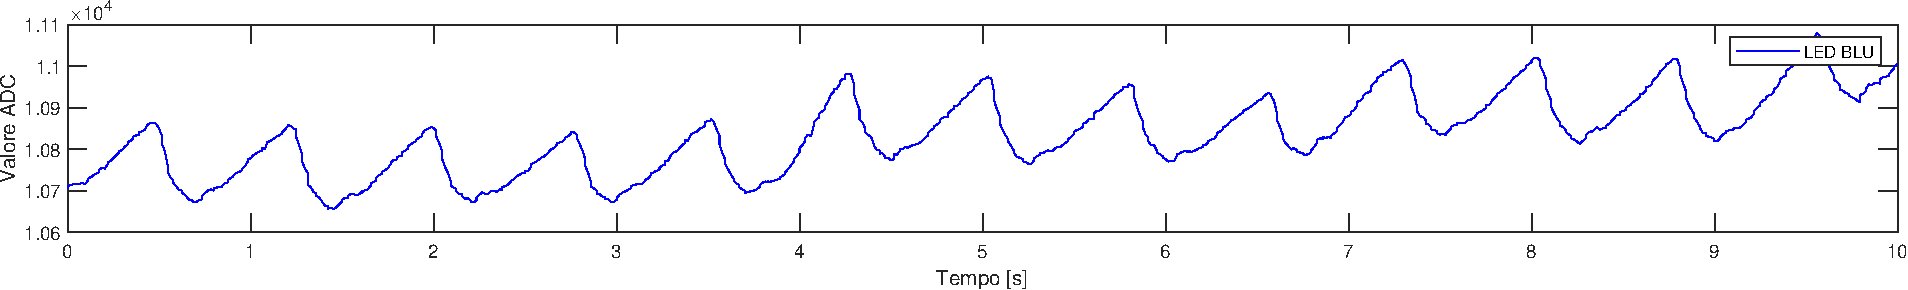
\includegraphics[width=1\linewidth]{ImageFiles/Misure Preliminari/Soggetto 1/MAX86916/lobo_blu}
	\caption{Soggetto 1 - Segnali PPG acquisiti sul lobo dell'orecchio destro con il sensore MAX86916.}
	\label{fig:soggetto1_MAX86916_lobo}
\end{figure}

\clearpage

\subparagraph{Polso antero-interno}

Si sono eseguite anche delle misure (\Fig~\ref{fig:soggetto1_MAX86916_polso}) sulla parte inferiore (antero-interna) del polso. Questa zona si è dimostrata essere molto influenzata dai movimenti del soggetto. I segnali del LED infrarosso e rosso risultano essere molto disturbati, sebbene siano ancora visibili i picchi caratteristici. I segnali dei LED verdi e blu risultano invece essere di buona qualità e il verde risulta avere l'ampiezza maggiore, sebbene minore delle acquisizioni effettuate sul lobo. La frequenza cardiaca che si può stimare è di 84 battiti al minuto.

\begin{figure}[h]
	\centering
	\includegraphics[width=1\linewidth]{ImageFiles/Misure Preliminari/Soggetto 1/MAX86916/polso_ired}
	\includegraphics[width=1\linewidth]{ImageFiles/Misure Preliminari/Soggetto 1/MAX86916/polso_red}
	\includegraphics[width=1\linewidth]{ImageFiles/Misure Preliminari/Soggetto 1/MAX86916/polso_green}
	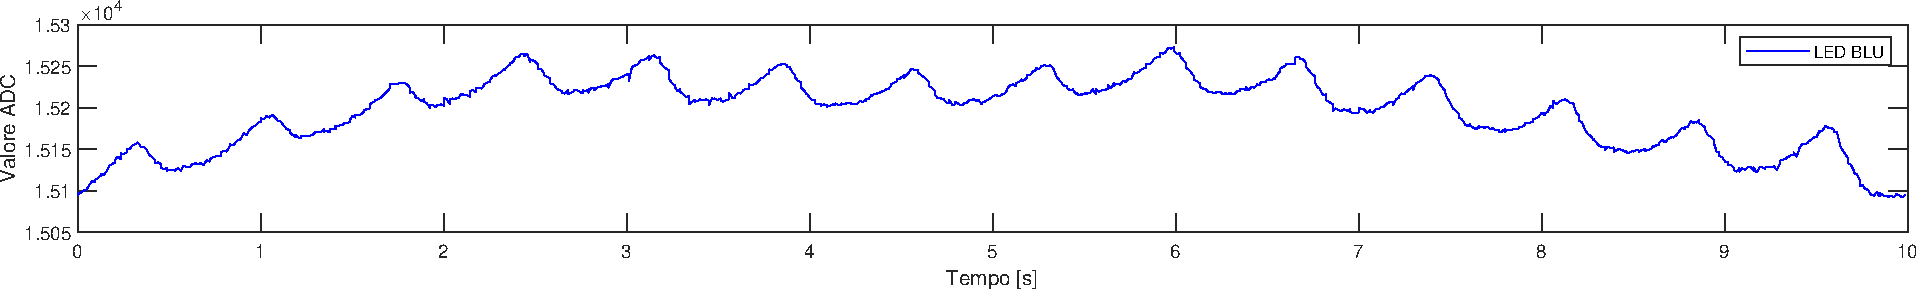
\includegraphics[width=1\linewidth]{ImageFiles/Misure Preliminari/Soggetto 1/MAX86916/polso_blu}
	\caption{Soggetto 1 - Segnali PPG acquisiti sul polso destro con il sensore MAX86916.}
	\label{fig:soggetto1_MAX86916_polso}
\end{figure}

\clearpage

\subparagraph{Fronte}

L'ultimo sito di misura analizzato è la fronte (\Fig~\ref{fig:soggetto1_MAX86916_fronte}). I segnali risultanti sono molto puliti ed è possibile notare i picchi sistolici in tutte le tracce. \textcolor{red}{Nel segnale dei} LED infrarosso e rosso è possibile notare anche il picco diastolico, mentre nei segnali relativi \textcolor{red}{ai} LED verde e blu, essi risultano esse impercettibili. La frequenza cardiaca rilevata è di 78 battiti al minuto. Questo sito è poco influenzato dai movimenti del soggetto e potrebbe essere utilizzato anche per misure durante l'attività fisica, ad esempio integrando il sensore in una fascia. L'ampiezza dei segnali ottenuti dai LED rosso e infrarosso sono superiori rispetto alle acquisizioni effettuate sul polso, ma l'ampiezza maggiore è ancora una volta ottenuta dal LED verde.

\begin{figure}[h]
	\centering
	\includegraphics[width=1\linewidth]{ImageFiles/Misure Preliminari/Soggetto 1/MAX86916/fronte_ired}
	\includegraphics[width=1\linewidth]{ImageFiles/Misure Preliminari/Soggetto 1/MAX86916/fronte_red}
	\includegraphics[width=1\linewidth]{ImageFiles/Misure Preliminari/Soggetto 1/MAX86916/fronte_green}
	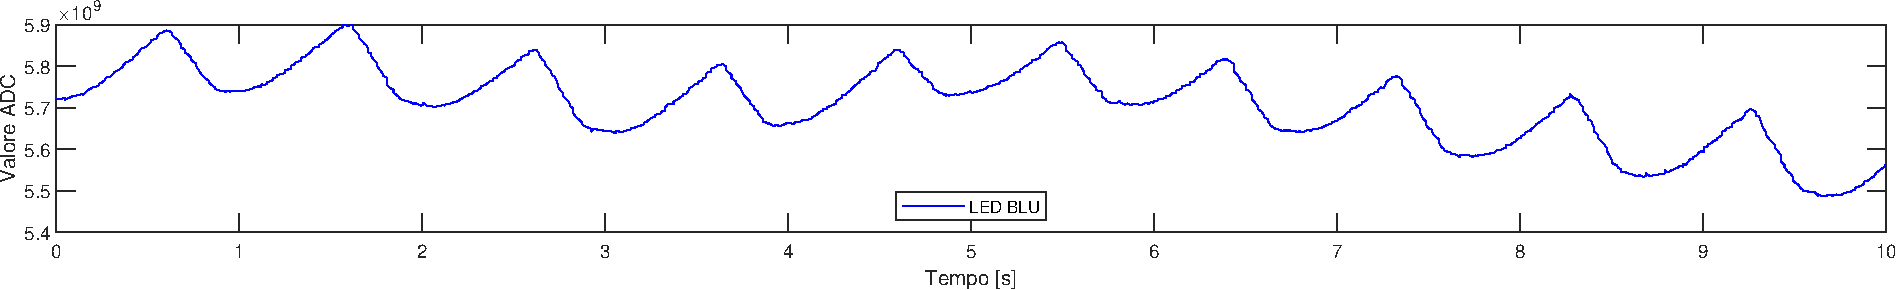
\includegraphics[width=1\linewidth]{ImageFiles/Misure Preliminari/Soggetto 1/MAX86916/fronte_blu}
	\caption{Soggetto 1 - Segnali PPG acquisiti sulla fronte con il sensore MAX86916.}
	\label{fig:soggetto1_MAX86916_fronte}
\end{figure}

\clearpage

Di seguito sono riportati i risultati ottenuti utilizzando il sensore \textbf{MAXM86161} su una finestra temporale di 10 secondi. Le immagini mostrano il segnale PPG filtrato grazie ad un filtro a media mobile.

\subparagraph{Polpastrello indice sinistro}

La figura \ref{fig:soggetto1_MAXM86161_polpastrello} mostra il segnale PPG acquisito e filtrato sul polpastrello del dito indice sinistro. Si è utilizzato un filtro a media mobile con finestra di 25 campioni per il LED verde  e di 20 per i LED rosso e infrarosso. In tutti e tre i campioni sono apprezzabili i picchi sistolici, anche se il segnale del LED rosso risulta essere di minore qualità, soprattutto dopo 8 secondi. Il segnale che presenta un valore AC maggiore è il verde, mentre il rosso risulta essere il segnale con minore ampiezza e più soggetto a disturbi. Osservando i segnali infrarosso e verde, che risultano più puliti, è possibile contare 13 picchi, suggerendo una frequenza cardiaca di circa 78 battiti.

\begin{figure}[h]
	\centering
	\includegraphics[width=1\linewidth]{ImageFiles/Misure Preliminari/Soggetto 1/MAXM86161/polpastrello_ired}
	\includegraphics[width=1\linewidth]{ImageFiles/Misure Preliminari/Soggetto 1/MAXM86161/polpastrello_red}
	\includegraphics[width=1\linewidth]{ImageFiles/Misure Preliminari/Soggetto 1/MAXM86161/polpastrello_green}
	\caption{Soggetto 1 - Segnali PPG acquisiti sul polpastrello del dito indice sinistro con il sensore MAXM86161.}
	\label{fig:soggetto1_MAXM86161_polpastrello}
\end{figure}

\clearpage

\subparagraph{Lobo orecchio destro}

Le acquisizioni effettuate sul lobo dell'orecchio destro (\Fig~\ref{fig:soggetto1_MAXM86161_polso}) sono state filtrate con una finestra di 20 campioni per il segnale a luce infrarossa e di 15 per i segnali dei LED verde e rosso. Come per i campioni acquisiti sul polpastrello, i segnali in cui è possibile osservare meglio i picchi sono \textcolor{red}{quelli dei LED} infrarosso e verde. In questa acquisizione il segnale ad ampiezza maggiore è quello dato dal LED infrarosso. Si può stimare una frequenza cardiaca di 84 battiti al minuto.

\begin{figure}[h]
	\centering
	\includegraphics[width=1\linewidth]{ImageFiles/Misure Preliminari/Soggetto 1/MAXM86161/lobo_ired}
	\includegraphics[width=1\linewidth]{ImageFiles/Misure Preliminari/Soggetto 1/MAXM86161/lobo_red}
	\includegraphics[width=1\linewidth]{ImageFiles/Misure Preliminari/Soggetto 1/MAXM86161/lobo_green}
	\caption{Soggetto 1 - Segnali PPG acquisiti sul lobo dell'orecchio destro con il sensore MAXM86161.}
	\label{fig:soggetto1_MAXM86161_lobo}
\end{figure}

\clearpage

\subparagraph{Polso antero-interno}

Le misure effettuate sul polso del soggetto, parte antero-interno, presentano una discreta qualità nelle misure dei LED verde(\Fig~\ref{fig:soggetto1_MAXM86161_polso}) e infrarosso. Quest'ultimo presenta l'ampiezza maggiore. Il segnale del LED rosso risulta essere un po' disturbato, sebbene, confrontandolo con il segnale verde, si possa notare una certa corrispondenza nei picchi. I segnali sono stati filtrati con un filtro a media mobile con finestra di  25 per l'infrarosso e di 20 per il rosso e verde. Nel tracciato del LED verde sono evidenti 15 picchi, che indicano un ritmo cardiaco del soggetto pari a 90 battiti al minuto.

\begin{figure}[h]
	\centering
	\includegraphics[width=1\linewidth]{ImageFiles/Misure Preliminari/Soggetto 1/MAXM86161/polso_ired}
	\includegraphics[width=1\linewidth]{ImageFiles/Misure Preliminari/Soggetto 1/MAXM86161/polso_red}
	\includegraphics[width=1\linewidth]{ImageFiles/Misure Preliminari/Soggetto 1/MAXM86161/polso_green}
	\caption{Soggetto 1 - Segnali PPG acquisiti sul polso destro con il sensore MAXM86161.}
	\label{fig:soggetto1_MAXM86161_polso}
\end{figure}

\clearpage

\subparagraph{Fronte}

I segnali acquisiti sulla fronte sono riportati nella figura \ref{fig:soggetto2_MAXM86161_fronte}. Per filtrare i dati è stato utilizzato un filtro con finestra di 20 per le acquisizioni dei LED infrarosso e rosso e di 10 per il segnale del LED verde. Come negli altri siti di misura, il LED rosso risulta avere un andamento più disturbato, mentre il segnale infrarosso e verde presentano una discreta qualità. I campioni della luce verde mostrano un andamento più liscio, mentre il segnale con ampiezza maggiore è quello della luce infrarossa. Dal tracciato del LED verde si possono facilmente contare 14 picchi sistolici, che equivalgono ad un ritmo cardiaco medio di 84 battiti al minuto.

\begin{figure}[h]
	\centering
	\includegraphics[width=1\linewidth]{ImageFiles/Misure Preliminari/Soggetto 1/MAXM86161/fronte_ired}
	\includegraphics[width=1\linewidth]{ImageFiles/Misure Preliminari/Soggetto 1/MAXM86161/fronte_red}
	\includegraphics[width=1\linewidth]{ImageFiles/Misure Preliminari/Soggetto 1/MAXM86161/fronte_green}
	\caption{Soggetto 1 - Segnali PPG acquisiti sulla fronte con il sensore MAXM86161.}
	\label{fig:soggetto1_MAXM86161_fronte}
\end{figure}




\clearpage